\chapter{The importance of temporal climate variability for spatial patterns in plant diversity}
\chaptermark{Temporal climate variability and plant diversity}

\graphicspath{{Chapter2/Figs/}}

\begin{center}

{\large Andrew D. Letten, Michael B. Ashcroft, David A. Keith, John R. Gollan and Daniel Ramp}

\small\textit{\textbf{Ecography}} \textbf{(2013), 36: 1341-1349}\\
\url{http://doi.wiley.com/10.1111/j.1600-0587.2013.00346.x}

\vspace{1in}

\includegraphics[width=0.15\linewidth]{Chapter2/Figs/mountain}

\vfill
This study was conceived by ADL with input from MAB, DAK, JRL \& DR. MAB and JRL collected climate data and modelled surfaces. ADL compiled floristic data, conducted analyses and wrote the manuscript, with contributions from MAB, DAK, JRL \& DR. 

\end{center}

\newpage
\section{Abstract}

Spatial variation in absolute climatic conditions (means, maxima or minima) is widely acknowledged to play a fundamental role in controlling species diversity patterns. In contrast, while evidence is accumulating that variability around mean climatic conditions may also influence species coexistence and persistence, the importance of spatial variation in temporal climatic variability for species diversity is still largely unknown. We used a unique dataset capturing fine-scale spatial heterogeneity in temperature variability across 2,490 plots in Southeast Australia to examine the comparative strength of absolute temperature and temperature variability in explaining spatial variation in plant diversity. Across all plots combined and in three of five forest types, temperature variability emerged as the better predictor of diversity. In all but one forest type, diversity also exhibited either a significant unimodal or positive linear correlation with temperature variability. This relationship is consistent with theory that predicts diversity will initially increase along a climate variability gradient due to temporal niche partitioning, but at an intermediary point, may decline as the risk of stochastic extinction exceeds competitive stabilization. These findings provide critical empirical evidence of a linkage between spatial variation in temporal climate variability and plant species diversity, and in light of changing climate variability regimes, highlight the need for ecologists to expand their purview beyond absolutes and averages.

\newpage
\section{Introduction}

Ecologists have long been interested in the role of environmental gradients in driving patterns of biodiversity \citep{Fox2011}. The relationship between species richness and spatial variation in climatic conditions, such as temperature and rainfall, has in particular received considerable attention \citep[e.g.][]{O'Brien1998, Currie2004, Kozak2012}. While the overarching emphasis has been on richness responses to spatial variation in mean (including maxima or minima) climate variables, recent evidence indicates that deterministic and stochastic elements of variability around mean climatic conditions may play an underappreciated role in species coexistence and persistence, and therefore in the maintenance of species diversity \citep{Chesson2000, Levine2004, Adler2006}. At the same time, the spectre of altered climatic variability regimes under future climates, including more frequent extreme weather events \citep{Easterling2000a, ippc2007, Hansen2012}, is providing an urgent mandate for ecologists to expand their purview beyond mean climate measures \citep{Adler2008, Shurin2010, White2010}.

At broad biogeographic scales, gradients in climatic means undoubtedly have a fundamental role in controlling richness gradients \citep{Francis2003}. But at the local scale, where ecological processes such as competition take increasing precedence, contemporary coexistence theory makes a salient argument for giving greater consideration to fluctuations around mean climate. Specifically, coexistence theory stipulates that under certain conditions variability can stabilize competition, and thus promote diversity, by increasing the number of temporal niches available within a fixed space (temporal niche partitioning) \citep{Chesson1997, Chesson2000}. Competitive stabilization occurs when competing species prosper under different conditions, and have the ability to `bank' fitness gains made during good times via what are termed `storage effects', such as long-lived adults or seed banks \citep{Chesson2000}. At the same time, it is widely recognised by practitioners of population viability analysis that too much environmental variability can be detrimental to population persistence because it reduces long-term population growth rates and increases vulnerability to stochastic extinction \citep{Alvarez2001, Boyce2006}. These differing perspectives make opposing predictions on the long-run trajectory of species diversity under climatic variability \citep{Levine2004}, but in some instances may be expected to generate a richness peak at intermediate levels of climate variability \citep{Adler2008}.

Unlike the rich body of literature providing evidence for broad scale richness-responses along mean climatic gradients \citep[as reviewed in][]{Pausas2001}, evidence relating temporal climate fluctuations to species coexistence and diversity has only recently begun to accumulate \citep{White2010}. The favoured approach has been to analyse historical population dynamics amongst coexisting plant species in temporally variable environments \citep{Levine2004, Adler2006, Adler2009, Angert2009}, but a small number of studies have employed alternative approaches including lab-based microcosm experiments \citep{Descamps-Julien2005, Jiang2007, Tuck2012} and comparative analyses of species richness across sites characterized by different levels of climate variability \citep{Shurin2010}. Notably, in their study of lake zooplankton communities, \citet{Shurin2010} demonstrated that richness increased with increasing temporal variability in water temperature and was more strongly correlated with variability than mean temperature. To our knowledge theirs is the only study to date to relate spatial variation in within-community species diversity to temporal climate variability.

In a recent review, \citet{White2010} highlighted the need for more comparative spatial studies on diversity-variability relationships to complement the traditional emphasis on population dynamics. A novel approach to testing diversity-variability relationships that reduces the confounding effects of large-scale climate patterns is to compare diversity at sites that share the same regional climate but exhibit heterogeneous temporal climate variability at the landscape-scale. For instance, organisms occupying a sheltered gully will typically experience less climatic variability, over various time-scales, than those inhabiting a nearby ridgeline. Capturing this fine-scale heterogeneity in climate variability across landscapes was until recently constrained by the limited availability of accurate climate data at fine spatial scales. Indeed, the coarse-scale grids routinely utilized by ecologists for modelling species distributions are inappropriate for this purpose because they are typically derived from data collected by standardized weather stations (i.e. sparsely distributed Stevenson screens positioned at ${\sim}$1.5--2 m on flat, cleared terrain) which are specifically designed to reduce the effects of landscape features, such as topographic shelter, that generate fine-scale heterogeneity \citep{Ashcroft2012b}. Fortunately, the availability of small, low-cost microclimatic sensors has made it more viable for researchers to produce fine-resolution climate surfaces that consider the effects of a much wider variety of climate forcing factors, including cold air drainage, topographic exposure and canopy cover \citep{Ashcroft2011, Ashcroft2012b}. With these sensors and methods it is possible to produce climate surfaces that are more tightly coupled to the conditions experienced by most organisms. 


Here we provide a unique analysis of the influence of temporal climate variability on species diversity in the terrestrial plant realm. To explore the relationship between temporal climate variability and plant diversity we assembled a dataset comprising more than 2,400 standardized floristic plots from temperate forests in Southeast Australia, together with fine-resolution climate grids derived from data collected over two years by near surface climate loggers \citep[see][]{Ashcroft2012b}. Our two main objectives were: (1) to compare the relative strength of temperature variability and absolute temperature, alongside other climate variables, as predictors of plant species diversity; and (2) to investigate the shape of the relationship between temperature variability and species diversity; i.e. does it exhibit consistency with either the predictions of coexistence theory (positive monotonic relationship), population viability theory (negative monotonic relationship) or a unified unimodal model \citep[\textit{sensu}][]{Adler2006}.

\section{Materials and Methods}

\subsection{Study area}

The study area comprises approximately 60,000 km2 in the Hunter Valley region of New South Wales, Australia (Fig. \ref{fig:studyarea}). Although parts of the region have been cleared or modified for agriculture and mining, there remain large patches of native vegetation within protected areas, including parts of two world heritage sites. These relatively undisturbed areas are topographically complex with an altitudinal range of more than 1,400m. The vegetation is dominated by dry and wet sclerophyll eucalypt forest, with smaller areas of heath, upland swamp, and temperate rainforest \citep{Keith2004}.

\begin{figure}[H]
\centering
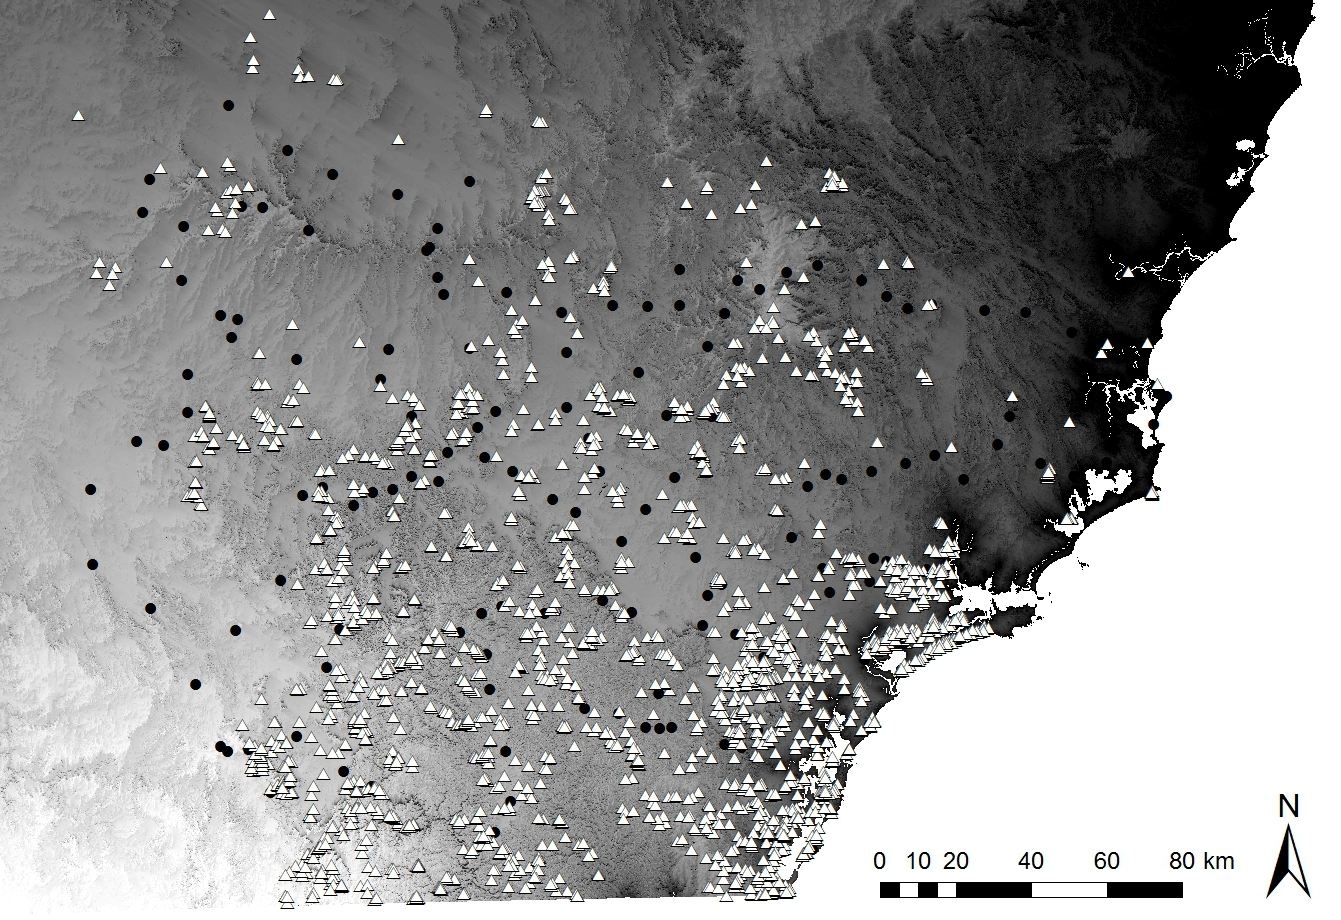
\includegraphics[width=1.0\linewidth]{./LettenetalEcographyRevision-img001}
\caption{Map of greater Hunter Valley study area (31.4--33.4{\textdegree}S, 149.4--152.6{\textdegree}E) showing locations of survey plots (white triangles) and climate loggers (black circles) overlaid on topoclimatic grid (25 x 25 m) of near-surface average variability in maximum temperature. Light to dark shading indicates transition from variable to stable localities. }
\label{fig:studyarea}
\end{figure}


\subsection{Floristic data}

Floristic data was assembled from the New South Wales Office and Environment and Heritage's YETI 3.2 vegetation plot database (\url{www.environment.nsw.gov.au/research/VISplot.htm}). Before performing analyses, the metadata for all surveys conducted in the study area were intensively scrutinized to ensure included records were from plots of a standard size (0.04 ha) and sampling effort; comprised a complete list of vascular plants; were accurately geo-referenced; and coincided geographically with regions mapped as native vegetation types on digitized maps. After implementing the evaluation criteria, a total of 2490 standardized 0.04 ha full-floristic plot records conducted between 1998 and 2010 were included in the analysis. 

Interspecific competition can occur between plants differing in size by several orders of magnitude. For instance, herbaceous species are known to limit the establishment of tree seedlings or even compete directly with adult trees \citep[e.g.][]{Riginos2009}. All vascular plants were therefore included in the assessment of species richness, which was quantified as the total number of species in each quadrat and ranged from 3 to 108 in any given plot, with a sum total of 2889 species representing 189 families. To evaluate whether observed response patterns varied across different growth-forms, supplementary analyses were performed on richness quantified for two separate groups: trees or arborescent shrubs; and all other growth-forms (hereafter trees and non-trees). Allotment of species into these groups was based on descriptions given in published floras \citep{Harden1993}, and may not reflect the actual growth form at a particular site. We performed all analyses on both the entire dataset and on subsets of the data grouped by forest type, which enabled us to explore whether the relationship between richness and climate variability varies between habitats, as has been shown for richness-disturbance relationships in wet vs. dry forests \citep{Bongers2009}.The exclusion of all forest types (derived from digitized maps) with less than 50 plots allowed for the partitioning of the data into five distinct forest types: grassy woodlands (GW; n = 225), dry sclerophyll forest (DSF; n = 1600), wet sclerophyll forest (WSF; n = 349), rainforest (RF; n = 101), and forested wetlands (FW; n = 215).

\subsection{Environmental data}

For the purposes of the study we refer to absolute temperature as any variable that provides an indication of the extreme or mean temperature at a site, but does not provide any indication of variability around extreme/mean temperature. For instance, two sites might have a mean annual temperature of 20 {\textdegree}C, but while one might experience relatively constant temperatures throughout the year, the other might fluctuate seasonally from a low of 5 {\textdegree}C to a high of 35 {\textdegree}C. Although there are a number of approaches to quantifying absolute temperature, we specifically focused on extreme temperature, rather than mean temperature, as extreme temperature is more tightly coupled with fine-scale topographical heterogeneity \citep{Suggitt2011}; is more likely to affect individual fitness than mean temperature \citep{Stenseth2002, Reyer2012}; and is predicted to fluctuate with greater frequency under climate change \citep{Smith2011}. As such, we defined absolute (extreme) temperature as the 95th percentile of daily maximum temperature and 5th percentile of daily minimum temperature over a one-year period.

For each quadrat location, temperature variables were extracted from a series of fine-resolution (25 m) topoclimatic grids interpolated from 113 climate loggers deployed within the study area for a total of 666 days from June 2009 to May 2011 (Fig. \ref{fig:studyarea}). To produce the grids of absolute temperature and temperature variability, the topoclimatic data was interpolated using a regional regression approach (Daly 2006), which involves fitting a multiple linear regression of temperature variables against climate-forcing factors including elevation, distance to coast, canopy cover, latitude, cold-air drainage, and topographic exposure \citep[see][for full details]{Ashcroft2011}. Variability in maximum temperature was initially partitioned into three time-scales: (i) intra-seasonal variation in maximum temperatures, calculated as the 95th percentile of summer (December--February) maximums minus the 5th percentile of summer maximums; (ii) intra-annual variation in maximum temperatures, calculated as the 95th percentile of summer (December--February) maximum temperatures minus the 95th percentile of winter (June--August) maximum temperatures; and (iii) inter-annual variation in maximum temperatures, calculated as the difference in the 95th percentile of maximum temperatures between the two years. In order to obtain a measure of overall variability in maximum temperature, we then calculated the average of the three variability grids at each locality \citep{Ashcroft2011, Ashcroft2012b}. To enable comparative analyses of temperature variability against other absolute climate variables, we also extracted the raw maximum and minimum temperature and humidity data (95th and 5th percentile of maximum and minimum temperatures) from the topoclimate surfaces, as well as five measures of rainfall derived from BioClim \citep{HoulderDHutchinsonMNixH2003}. Given that variability in minimum temperature was strongly correlated with absolute climate factors, we constrained our measure of variability to variability in maximum temperatures, while also controlling for potential direct effects of canopy cover on species richness by including remotely sensed canopy cover estimates \citep{DECC2008} as covariables in the multiple predictor models. The complete list of variables is provided in (Table \ref{tab:vars}). All explanatory variables were Z-standardized. 

\begin{flushleft}
\begin{table}
\renewcommand{\arraystretch}{1.2}
\caption{\footnotesize Factors available for selection as correlates of species richness in multi-variable models.}
\scriptsize
\begin{tabular}{m{3.4in}m{0.7in}m{1.3in}}
\hline
Variable &
Abbreviation &
Source\\\hline
Average variability in 95th percentile of maximum temperature &
VarMT &
Ashcroft et al., 2012\\
95th percentile of maximum temperature &
MaxT95 &
Ashcroft \& Gollan, 2011\\
5th percentile of maximum temperature &
MaxT5 &
Ashcroft \& Gollan, 2011\\
95th percentile of minimum temperature &
MinT95 &
Ashcroft \& Gollan, 2011\\
5th percentile of minimum temperature &
MinT5 &
Ashcroft \& Gollan, 2011\\
95th percentile of maximum humidity &
MaxH95 &
Ashcroft \& Gollan, 2011\\
5th percentile of maximum humidity &
MaxH5 &
Ashcroft \& Gollan, 2011\\
95th percentile of minimum humidity &
MinH95 &
Ashcroft \& Gollan, 2011\\
5th percentile of minimum humidity &
MinH5 &
Ashcroft \& Gollan, 2011\\
Mean annual precipitation &
AP &
Bioclim\\
Precipitation of warmest quarter &
PWaQ &
Bioclim\\
Precipitation of coldest quarter &
PCQ &
Bioclim\\
Precipitation of driest quarter &
PDQ &
Bioclim\\
Precipitation of wettest quarter &
PWeQ &
Bioclim\\
Canopy cover &
CC &
DECC, 2008\\\hline
\end{tabular}
\label{tab:vars}
\end{table}
\end{flushleft}

\subsection{Analysis}

In order to provide a direct comparison between temperature variability and absolute temperature as predictors of plant species richness (Objective 1), we first fitted single-predictor generalized linear models (GLMs) for species richness as a quadratic and a linear function of each of average variability in maximum temperatures and the 95th percentile of maximum temperatures. This simultaneously enabled us to investigate the shape of the relationship between species richness and climate variability in each forest type (Objective 2). The models were initially fitted with Poisson error-distributions to account for the strictly non-normal distribution of count data, but due to overdispersion (variance {\textgreater} mean) we subsequently corrected the standard errors using a quasi-Poisson GLM model. For all significant quadratic and linear terms, we calculated the quasi-AIC (QAIC) value, a modification of AIC based on quasi-likelihood appropriate for overdispersed response variables \citep{Burn}, and the percent deviance explained by the model as: [1 -- (observed deviance - residual deviance)] x 100. If both linear and quadratic models showed statistical significance, we chose the model with the lowest QAIC value (using the dispersion parameter derived from the global quadratic model). 

To determine how important temperature variability was, compared to other climate variables in predicting species richness patterns across the different forest types, we employed a multi-model information theoretic approach \citep{Burn}. The explanatory variables available for inclusion in the master model were first selected from the pool of climate variables (plus canopy cover) in Table \ref{tab:vars}. Prior to model selection, independent relationships (linear and quadratic) between species richness and each potential explanatory variable were evaluated for significance. To mitigate the problematic effects of collinearity in explanatory variables \citep{Dormann2012}, we evaluated correlations between all significant variables. Wherever two variables were strongly correlated (Pearson's {\textbar}r{\textbar} {\textgreater} 0.7), we excluded the variable exhibiting the weakest (greater QAIC) independent relationship with species richness. 

Model selection was performed using the dredge function in the R package `MuMIN' \citep{Barton2012}, whereby GLMs with quasi-Poisson error distributions were run for all variable combinations in each forest type and were evaluated and ranked according to their QAIC. We intentionally employed such an indiscriminate method in order to make any inference on the relationship between temperature variability (1 factor), versus absolute climate variables (14 factors) (Table \ref{tab:vars}), and species richness as conservative as possible. That is to say our approach ensured we would only conclude there was a significant relationship between richness and temperature variability if no other factors could explain this trend.

To evaluate the predictive power of each explanatory variable, we first constructed a 95\% confidence set of models for each forest type by summing the cumulative Akaike weights, $w_{i}$, of the highest ranked models until the sum exceeded 0.95. The relative importance of each variable was then calculated as the sum of the Akaike weights `$w_{+}(j)$' for all the models in which the variable of interest occurred in the 95\% confidence set. Model averaging was finally applied to determine model averaged parameter coefficients for the 95\% confidence set of models in each forest type \citep{Burn}.


Given the spatially clustered nature of some of the quadrats, we tested for spatial autocorrelation using Moran's I tests. Moran's I tests revealed significant autocorrelation in the residuals of the global models for each habitat type. While there a number of methods for dealing with spatial auto-correlation in normally distributed data, the available methods for dealing with non-normal data are more limited, and either suffer from a lack of precision in their ability to accurately estimate model coefficients \citep{Dormann2007}, or have only been tested on a limited number of datasets \citep{Murphy2010}. However, because the coefficients obtained in our models are almost identical to those obtained assuming normally distributed data (Table S2.1), we were satisfied that running simultaneous autoregressive (SAR) models, an effective approach to removing spatial autocorrelation from residuals assuming normal error distributions \citep{Kissling2007}, would provide a valid test of the effect of spatial autocorrelation on the model results. SAR models were generated using the R package `spdep' (Bivand 2012).

\section{Results}

The percentage variation in species richness explained by temperature variability in the single-predictor models followed an increasing trend from the driest to the wettest (based on annual precipitation) forest types (Table \ref{tab:temp}, Appendix A, Fig. S2.1). Variability in maximum temperature performed better (greater explanatory power) than absolute maximum temperature as a univariate predictor of species richness in all plots combined and in the three wetter forest types but performed poorer in the two driest forest types: grassy woodland and dry sclerophyll forest (Table \ref{tab:vars}). Species richness exhibited a significant (P {\textless} 0.05) unimodal relationship with temperature variability across all plots combined and across all individual forest types, with the exception of forested wetlands and grassy woodlands, which showed a significant positive linear relationship and no relationship respectively (Fig. \ref{fig:humpplots}). Relative performance of the two temperature metrics in predicting tree species richness were similar to those described for all vascular plants in each of the five different forest types, but in all plots combined absolute temperature performed better than temperature variability (12.8 vs. 5.1 percentage deviance explained) (Table S2.4). For all non-tree species, patterns were again similar to those observed for all vascular plants, with the exception of dry sclerophyll forest and rainforest, where there was very little difference in performance between absolute temperature and temperature variability (Table S2.5).

\begin{flushleft}
\begin{table}[H]
\renewcommand{\arraystretch}{1.2}
\caption{\footnotesize Percentage deviance explained by variability in maximum temperature (VarMT) and absolute maximum temperature (MaxT95) as independent predictors of species richness, and the range of percentage deviance explained in the 95\% confidence set of multiple predictor models for each forest type and all plots combined (ALL = all plots combined, DSF = dry sclerophyll forest, WSF = wet sclerophyll forest, GW = grassy woodland, RF = rainforest \ and FW = forested wetlands). \ Non-significant results are shown in brackets. The ratio VarMT/MaxT95 provides a measure of the relative explanatory power of temperature variability and absolute temperature.}
\scriptsize
\begin{tabular}{m{0.4in}m{0.7in}m{0.7in}m{1.5in}m{1.6in}}
\hline
~
 &
\multicolumn{2}{m{1.6851599in}}{\centering Single-predictor models} &
\centering Relative explanatory power &
\centering\arraybackslash Multiple-predictor models\\
~ &
\centering VarMT &
\centering MaxT95 &
\centering (VarMT/MaxT95) &
\centering\arraybackslash 95\% confidence set *\\\hline
ALL &
\centering 4.85 &
\centering 1.00 &
\centering 4.9 &
\centering\arraybackslash 16.19 - 16.49\\
GW &
\centering (0.64) &
\centering 6.56 &
\centering 0.1 &
\centering\arraybackslash 11.11 - 12.03\\
DSF &
\centering 1.94 &
\centering 3.32 &
\centering 0.6 &
\centering\arraybackslash 17.35 - 17.61\\
WSF &
\centering 10.32 &
\centering 3.63 &
\centering 2.8 &
\centering\arraybackslash 13.50 - 16.82\\
RF &
\centering 13.03 &
\centering (4.65) &
\centering 2.9 &
\centering\arraybackslash 29.35 - 38.15\\
FW &
\centering 19.28 &
\centering 10.90 &
\centering 1.8 &
\centering\arraybackslash 26.27 \ {}- 31.10\\\hline
\multicolumn{5}{l}{* see Table S2.3 for models comprising the 95\% confidence set.}
\end{tabular}
\label{tab:temp}
\end{table}
\end{flushleft}

As is to be expected, a number of the climate variables available for model selection were highly correlated ({\textbar}r{\textbar} {\textgreater} 0.7), necessitating the exclusion of the weaker ({\textgreater}QAIC) of each collinear pair (Table S2.2). Variability in maximum temperature generally exhibited weak to moderate collinearity with the other variables, but in dry sclerophyll forest it was strongly negatively correlated with the 95th percentile of minimum temperature (r = -0.704), while in forested wetlands it was strongly negatively correlated with both precipitation of the driest quarter (r = -0.746) and precipitation of the coldest quarter (r = -0.734). In each instance, variability in maximum temperature exhibited the lowest QAIC and thus was retained.

\begin{figure}[H]
\centering
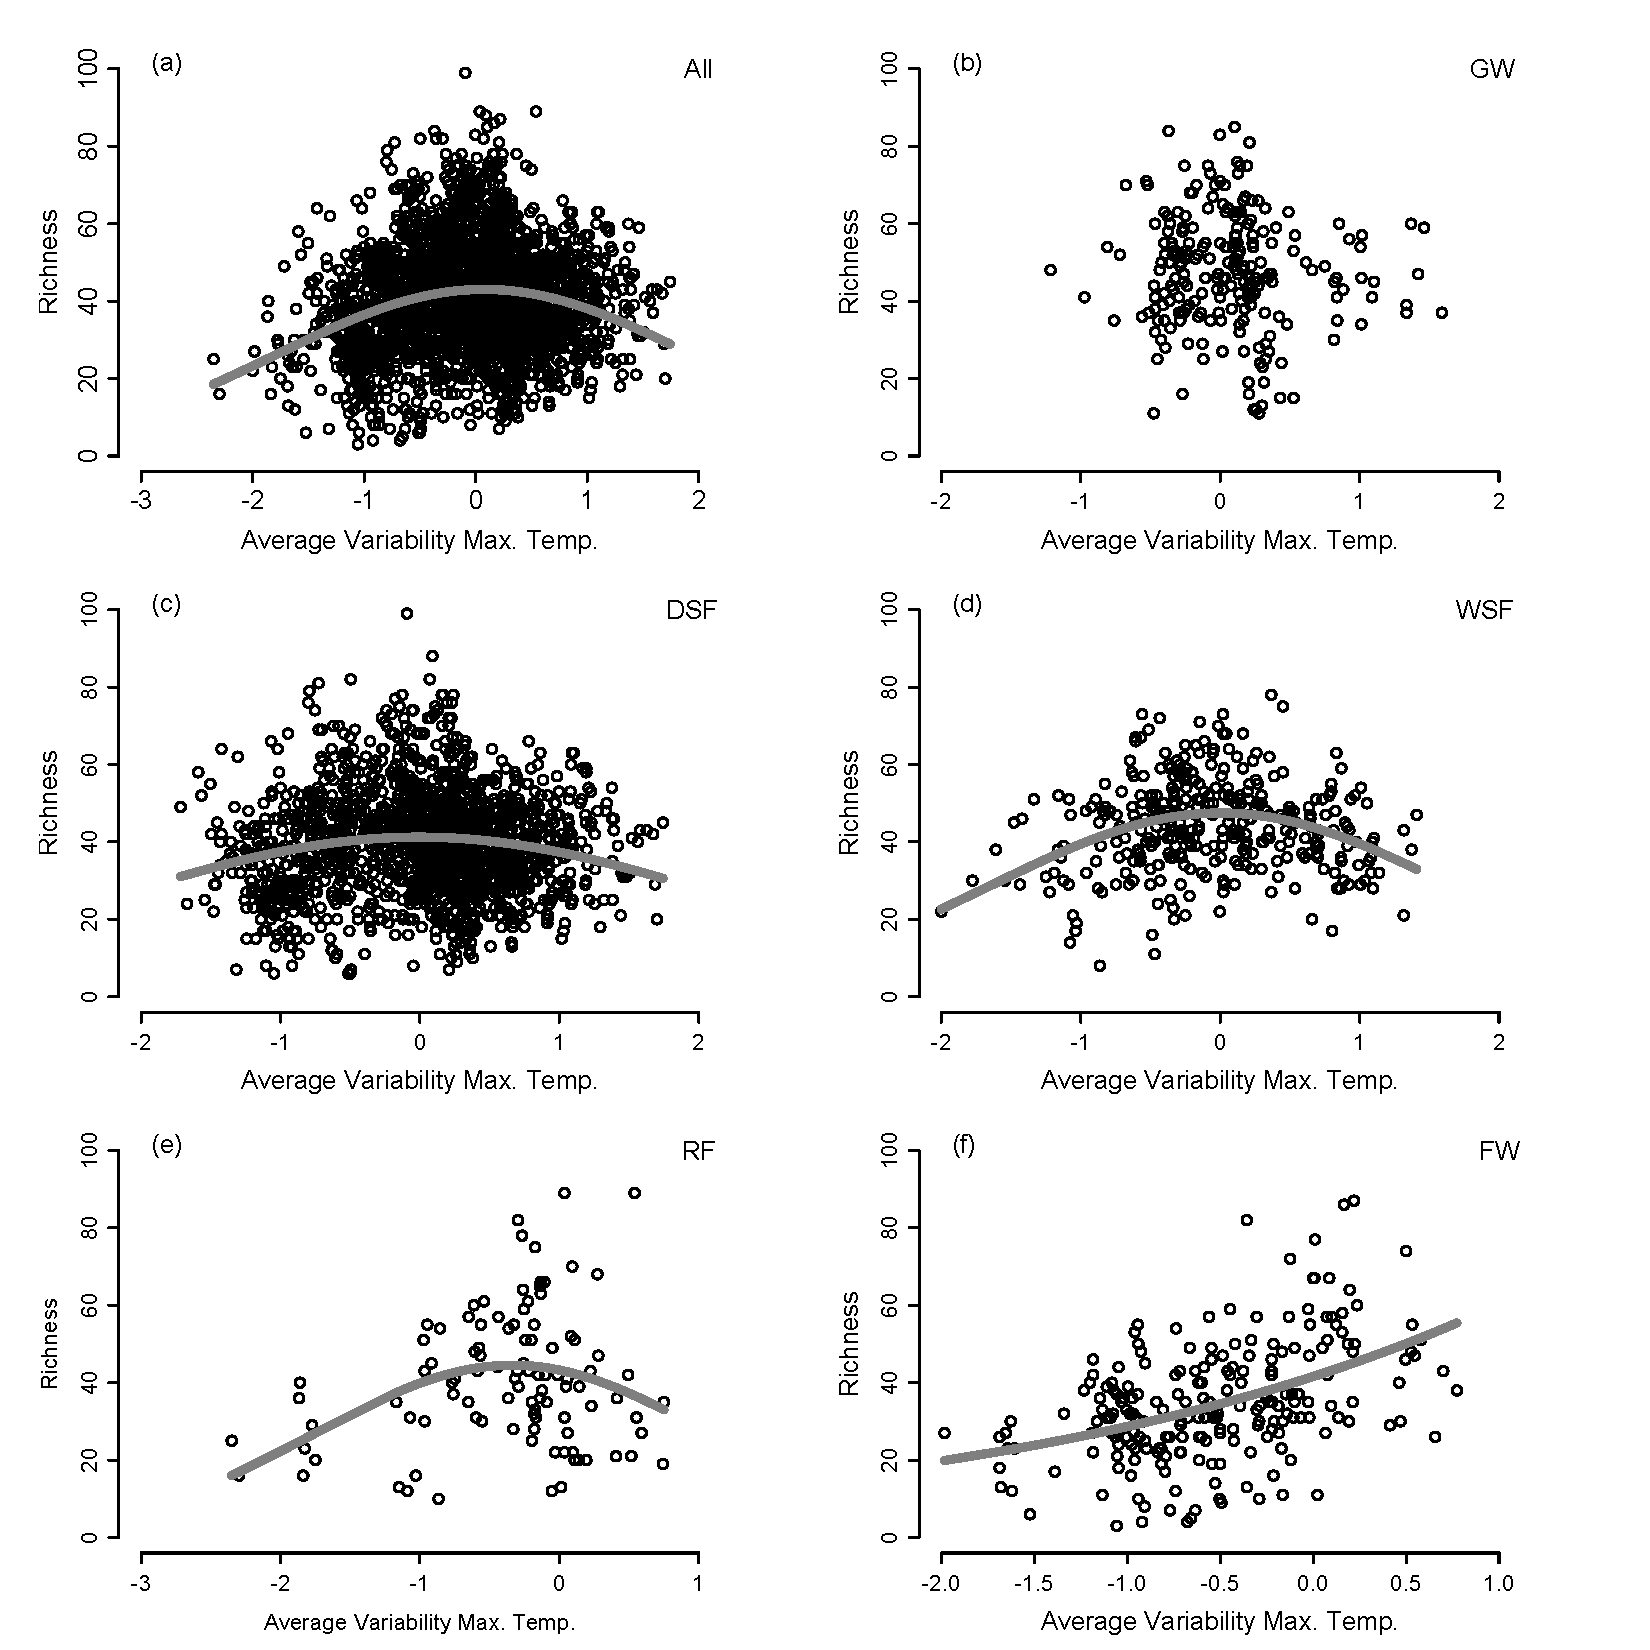
\includegraphics[width=0.85\linewidth]{./thesisversionFig2}
\caption{Relationship between species richness and average variability in maximum temperature (VarMT) in: all plots combined (ALL, n = 2490) (a), grassy woodland (GW, n = 255) (b), dry sclerophyll forest (DSF, n = 1600) (c), wet sclerophyll forest (WSF, n = 349) (d), rainforest (RF, n = 101) (e), and forested wetlands (FW, n = 215) (f). Solid grey lines are the lines of best fit for significant single-predictor GLMs (linear model in FW exhibits slight upward curvature due to log-link function of Poisson regression). Percentage deviance explained by each model is given in Table 2.2.}
\label{fig:humpplots}
\end{figure}


In the multiple-predictor models, variability in maximum temperature emerged as an important predictor of species richness relative to the absolute climate variables across all plots combined and in all forest types with the exception of grassy woodlands (Table \ref{tab:coefs}, Table S2.3). In particular, variability in maximum temperatures was the single most important climate variable explaining species richness in wet sclerophyll forests, and the joint most important variable (together with the 5th percentile of maximum humidity) in forested wetlands. In rainforest, variability in maximum temperature was the joint third most important variable, while in dry sclerophyll forest and all plots combined, almost all the variables, including variability in maximum temperature, occurred in the 95\% confidence set of best models. 

\begin{flushleft}
\begin{table}[t]
\renewcommand{\arraystretch}{1.2}
\caption{\footnotesize Coefficient estimates, standard errors and associated P{}-values (*P {\textless} 0.05, **P {\textless} 0.01, ***P {\textless} 0.001) of model averaged parameters in the 95\% confidence set for each forest type. Summed Akaike weights [$w_{+}(j)$] provide a measure of the importance of each covariate. (ALL = all plots combined, DSF = dry sclerophyll forest, WSF = wet sclerophyll forest, GW = grassy woodland, RF = rainforest \ and FW = forested wetlands.}
\scriptsize
\begin{tabular}{m{0.4in}m{0.3in}m{0.15in}m{0.05in}m{0.1in}m{0.01in}m{0.4in}m{0.3in}m{0.15in}m{0.05in}m{0.1in}m{0.01in}m{0.4in}m{0.3in}m{0.15in}m{0.05in}m{0.1in}}
\hline
ALL &
~ &
~ &
~ &
~ &
~ &
GW &
~ &
~ &
~ &
~ &
~ &
DSF &
~ &
~ &
~ &
~\\
Variable &
\centering Estimate &
\centering SE &
\centering P &
\centering w+(j) &
\centering ~ &
Variable &
\centering Estimate &
\centering SE &
\centering P &
\centering w+(j) &
~ &
Variable &
\centering Estimate &
\centering SE &
\centering P &
\centering\arraybackslash w+(j)\\\hline
\textbf{VarMT} &
\centering \textbf{1.45} &
\centering \textbf{0.33} &
\centering *** &
\centering ~ &
\centering ~ &
PWaQ &
\centering {}-0.79 &
\centering 0.22 &
\centering *** &
\centering ~ &
~ &
\textbf{VarMT }&
\centering \textbf{0.02} &
\centering \textbf{0.32} &
\centering ~ &
\centering\arraybackslash ~\\
\textbf{VarMT$^{2}$} &
\centering \textbf{{}-2.61} &
\centering \textbf{0.22} &
\centering *** &
\centering \textbf{1.00} &
\centering ~ &
PWaQ$^{2}$ &
\centering {}-1.61 &
\centering 0.20 &
\centering *** &
\centering 1.00 &
~ &
\textbf{VarMT$^{2}$} &
\centering \textbf{{}-1.51} &
\centering \textbf{0.20} &
\centering *** &
\centering\arraybackslash \textbf{1.00}\\
MinT5 &
\centering {}-2.84 &
\centering 0.45 &
\centering *** &
\centering ~ &
\centering ~ &
MinT5 &
\centering 0.45 &
\centering 0.18 &
\centering * &
\centering ~ &
~ &
MinT5 &
\centering 0.16 &
\centering 0.33 &
\centering ~ &
\centering\arraybackslash ~\\
MinT5$^{2}$ &
\centering 2.21 &
\centering 0.18 &
\centering *** &
\centering 1.00 &
\centering ~ &
MinT5$^{2}$ &
\centering {}-0.14 &
\centering 0.18 &
\centering ~ &
\centering 0.20 &
~ &
MinT5$^{2}$ &
\centering 1.55 &
\centering 0.17 &
\centering *** &
\centering\arraybackslash 1.00\\
MinT95 &
\centering 3.61 &
\centering 0.51 &
\centering *** &
\centering ~ &
\centering ~ &
MaxH5 &
\centering {}-0.29 &
\centering 0.19 &
\centering ~ &
\centering ~ &
~ &
MaxH5 &
\centering {}-0.40 &
\centering 0.30 &
\centering ~ &
\centering\arraybackslash ~\\
MinT95$^{2}$ &
\centering {}-0.01 &
\centering 0.37 &
\centering ~ &
\centering 1.00 &
\centering ~ &
MaxH5$^{2}$ &
\centering 0.09 &
\centering 0.18 &
\centering ~ &
\centering 0.16 &
~ &
MaxH5$^{2}$ &
\centering {}-1.74 &
\centering 0.20 &
\centering *** &
\centering\arraybackslash 1.00\\
MaxH5 &
\centering {}-3.47 &
\centering 0.47 &
\centering *** &
\centering ~ &
\centering ~ &
MaxH95 &
\centering {}-0.41 &
\centering 0.22 &
\centering . &
\centering ~ &
~ &
MaxH95 &
\centering {}-0.72 &
\centering 0.29 &
\centering * &
\centering\arraybackslash ~\\
MaxH5$^{2}$ &
\centering {}-2.77 &
\centering 0.21 &
\centering *** &
\centering 1.00 &
\centering ~ &
MaxH95$^{2}$ &
\centering {}-0.17 &
\centering 0.23 &
\centering ~ &
\centering 0.11 &
~ &
MaxH95$^{2}$ &
\centering {}-1.59 &
\centering 0.19 &
\centering *** &
\centering\arraybackslash 1.00\\
MaxH95 &
\centering 0.76 &
\centering 0.39 &
\centering . &
\centering ~ &
\centering ~ &
\centering ~ &
\centering ~ &
\centering ~ &
\centering ~ &
\centering ~ &
~ &
MinH5 &
\centering 1.88 &
\centering 0.44 &
\centering *** &
\centering\arraybackslash ~\\
MaxH95$^{2}$ &
\centering {}-0.66 &
\centering 0.26 &
\centering * &
\centering 0.43 &
\centering ~ &
\centering ~ &
\centering ~ &
\centering ~ &
\centering ~ &
\centering ~ &
~ &
MinH5$^{2}$ &
\centering {}-1.19 &
\centering 0.22 &
\centering *** &
\centering\arraybackslash 1.00\\
MinH5 &
\centering 2.91 &
\centering 0.43 &
\centering *** &
\centering ~ &
\centering ~ &
\centering ~ &
\centering ~ &
\centering ~ &
\centering ~ &
\centering ~ &
~ &
PCQ &
\centering {}-0.91 &
\centering 0.36 &
\centering * &
\centering\arraybackslash ~\\
MinH5$^{2}$ &
\centering {}-1.80 &
\centering 0.24 &
\centering *** &
\centering 1.00 &
\centering ~ &
\centering ~ &
\centering ~ &
\centering ~ &
\centering ~ &
\centering ~ &
~ &
PCQ$^{2}$ &
\centering {}-2.73 &
\centering 0.24 &
\centering *** &
\centering\arraybackslash 1.00\\
PCQ &
\centering {}-0.52 &
\centering 0.38 &
\centering ~ &
\centering ~ &
\centering ~ &
\centering ~ &
\centering ~ &
\centering ~ &
\centering ~ &
\centering ~ &
~ &
CC &
\centering 1.02 &
\centering 0.23 &
\centering *** &
\centering\arraybackslash 0.83\\
PCQ$^{2}$ &
\centering {}-4.00 &
\centering 0.23 &
\centering *** &
\centering 1.00 &
\centering ~ &
\centering ~ &
\centering ~ &
\centering ~ &
\centering ~ &
\centering ~ &
~ &
~ &
~ &
~ &
~ &
~\\
CC &
\centering 1.07 &
\centering 0.23 &
\centering *** &
\centering 0.86 &
\centering ~ &
\centering ~ &
\centering ~ &
\centering ~ &
\centering ~ &
\centering ~ &
~ &
~ &
~ &
~ &
~ &
~\\
~ &
~ &
~ &
~ &
~ &
~ &
~ &
~ &
~ &
~ &
~ &
~ &
~ &
~ &
~ &
~ &
~\\
WSF \  &
~ &
~ &
~ &
~ &
~ &
RF &
~ &
~ &
~ &
~ &
~ &
FW &
~ &
~ &
~ &
~\\
Variable &
\centering Estimate &
\centering SE &
\centering P &
\centering w+(j) &
\centering ~ &
Variable &
\centering Estimate &
\centering SE &
\centering P &
\centering w+(j) &
\centering ~ &
Variable &
\centering Estimate &
\centering SE &
\centering P &
\centering\arraybackslash w+(j)\\\hline
\textbf{VarMT} &
\centering \textbf{0.25} &
\centering \textbf{0.24} &
\centering ~ &
\centering ~ &
~ &
MaxH95 &
\centering 0.84 &
\centering 0.46 &
\centering . &
\centering ~ &
~ &
\textbf{VarMT} &
\centering \textbf{2.01} &
\centering \textbf{0.31} &
\centering *** &
\centering\arraybackslash \textbf{1.00}\\
\textbf{VarMT$^{2}$} &
\centering \textbf{{}-1.60} &
\centering \textbf{0.20} &
\centering *** &
\centering \textbf{1.00} &
~ &
MaxH95$^{2}$ &
\centering {}-1.51 &
\centering 0.65 &
\centering * &
\centering 0.82 &
~ &
MaxH5 &
\centering {}-1.98 &
\centering 0.27 &
\centering *** &
\centering\arraybackslash ~\\
PDQ &
\centering {}-0.64 &
\centering 0.23 &
\centering ** &
\centering ~ &
~ &
MinT95 &
\centering 1.64 &
\centering 0.39 &
\centering *** &
\centering ~ &
~ &
MaxH5$^{2}$ &
\centering {}-1.44 &
\centering 0.25 &
\centering *** &
\centering\arraybackslash 1.00\\
PDQ2 &
\centering {}-0.74 &
\centering 0.19 &
\centering *** &
\centering 0.98 &
~ &
MinT95$^{2}$ &
\centering {}-1.48 &
\centering 0.36 &
\centering *** &
\centering 0.76 &
~ &
MinT95 &
\centering 1.32 &
\centering 0.35 &
\centering *** &
\centering\arraybackslash ~\\
MaxT5 &
\centering 0.14 &
\centering 0.28 &
\centering ~ &
\centering ~ &
~ &
\textbf{VarMT} &
\centering \textbf{1.04} &
\centering \textbf{0.52} &
\centering * &
\centering ~ &
~ &
MinT95$^{2}$ &
\centering {}-0.28 &
\centering 0.19 &
\centering ~ &
\centering\arraybackslash 0.87\\
MaxT5$^{2}$ &
\centering {}-0.67 &
\centering 0.20 &
\centering ** &
\centering 0.56 &
~ &
\textbf{VarMT$^{2}$} &
\centering \textbf{{}-0.55} &
\centering \textbf{0.23} &
\centering * &
\centering \textbf{0.45} &
~ &
MaxH95 &
\centering 1.34 &
\centering 0.33 &
\centering *** &
\centering\arraybackslash 0.81\\
MaxT95 &
\centering 0.08 &
\centering 0.29 &
\centering ~ &
\centering ~ &
~ &
PDQ &
\centering {}-0.01 &
\centering 0.42 &
\centering ~ &
\centering ~ &
~ &
AP &
\centering 0.21 &
\centering 0.38 &
\centering ~ &
\centering\arraybackslash 0.28\\
MaxT95$^{2}$ &
\centering {}-0.56 &
\centering 0.21 &
\centering ** &
\centering 0.40 &
~ &
PDQ$^{2}$ &
\centering {}-1.01 &
\centering 0.31 &
\centering ** &
\centering 0.45 &
~ &
MinH5 &
\centering 0.79 &
\centering 0.55 &
\centering ~ &
\centering\arraybackslash ~\\
MinH95 &
\centering 0.17 &
\centering 0.18 &
\centering ~ &
\centering ~ &
~ &
MinH5 &
\centering 0.70 &
\centering 0.41 &
\centering . &
\centering ~ &
~ &
MinH5$^{2}$ &
\centering {}-0.15 &
\centering 0.22 &
\centering ~ &
\centering\arraybackslash 0.23\\
MinH95$^{2}$ &
\centering {}-0.40 &
\centering 0.18 &
\centering * &
\centering 0.31 &
~ &
MinH5$^{2}$ &
\centering {}-0.01 &
\centering 0.23 &
\centering ~ &
\centering 0.20 &
~ &
MaxT95 &
\centering 0.83 &
\centering 0.67 &
\centering ~ &
\centering\arraybackslash ~\\
MinT5 &
\centering 0.10 &
\centering 0.22 &
\centering ~ &
\centering ~ &
~ &
~ &
~ &
~ &
~ &
~ &
~ &
MaxT95$^{2}$ &
\centering 0.14 &
\centering 0.21 &
\centering ~ &
\centering\arraybackslash 0.22\\
MinT5$^{2}$ &
\centering {}-0.07 &
\centering 0.18 &
\centering ~ &
\centering 0.11 &
~ &
~ &
~ &
~ &
~ &
~ &
~ &
~ &
\centering\arraybackslash ~\\\hline
\end{tabular}
\label{tab:coefs}
\end{table}
\end{flushleft}
In support of the single-predictor models, coefficient estimates derived from model averaging confirmed that species richness was consistently best modelled as a significant negative quadratic function of variability in maximum temperature in three of five forest types, as well as the combined data. Exceptions were forested wetlands, for which variability in maximum temperature was consistently positive and linear, and grassy woodlands where non-significant univariate models precluded the inclusion of variability in maximum temperature in the model selection process.

The global models for all forest types and all plots combined exhibited significant spatial correlation in the residuals. However, parameter estimates obtained with spatial regression models (SAR error models) were almost identical in sign and significance to those obtained with non-spatial GLMs (Table S2.1). In particular, the sign and significance of the linear and quadratic terms for variability in maximum temperature were consistent across almost all global models, regardless of whether the models were regressed using a non-spatial quasi-Poisson model, a non-spatial Gaussian model or a spatially sensitive SAR error model. The only exception was for dry sclerophyll forest where the quadratic term for variability in maximum temperature was no longer significant when modelled using SAR models. We therefore concluded that the results were largely insensitive to spatial autocorrelation in the data.


\section{Discussion}

The results of this study provide novel evidence that at local spatial scales temperature variability may be a better predictor of plant species diversity than absolute measures of temperature such as means, maxima, or minima. Specifically, our most important finding was that across all plots combined and in three of five individual forest types, the explanatory power of temperature variability was in the order of around two to five times that of absolute temperature (Table \ref{tab:temp}). This relationship supports the contention that spatial variation in temporal temperature variability plays a more important role in regulating species coexistence and persistence than comparative spatial variation in absolute temperature. In a previous study that compared diversity patterns across localities differing in their temporal climate variability profile, \citet{Shurin2010} similarly found that variation in freshwater zooplankton richness was better explained by temperature variability than mean temperature. To our knowledge these results provide the first empirical evidence of a linkage between spatial variation in temporal climate variability and plant species diversity at local scales.


It is instructive that in both the single- and multiple-predictor models the performance of temperature variability as a predictor of plant diversity increased from the driest to the wettest forest types, which would suggest that temperature variability has a more crucial role in structuring plant communities where water is non-limiting. However, given that absolute temperature also performed poorly as a predictor of species richness in the drier forest types, we cannot rule out the possibility of higher level water-energy dynamics precluding richness responses to temperature in dry habitats \citep{Francis2003}. It is also likely that the greater frequency of fires in dry forest types \citep{CLARKE2005} supersedes the influence of climatic factors, such as temperature, on species richness patterns. Indeed, the best multiple-predictor models for grassy woodlands, the driest vegetation type in our study, were poorer than all other forest types in explaining variation in species richness, suggesting that climate factors in general may have a less important role in structuring plant communities in drier habitats. Notably, \citet{Bongers2009} found that a disturbance index integrating primarily non-climatic variables such as logging and fire was better at explaining variation in tree species diversity in dry forest types than in wet forest types. This is consistent with our findings that climatic factors appear to be less important drivers of richness patterns in dry habitats than mesic habitats. 


The statistically strong independent relationship between temperature variability and species richness for all forest types combined is counterbalanced by weak explanatory power (4.85\%), albeit within the range typical of many ecological studies \citep{Jennions2002} and almost five times that explained by absolute temperature. One plausible explanation is that factors other than temperature variability exert a stronger influence on species richness in our study area. A number of \ variables that were not included in the models may be expected to exert a substantial influence on fine-scale richness patterns, including soil and nutrient profiles, water availability, fire frequency, logging history and other forms of anthropogenic disturbance \citep{Pausas2001}. It is also possible that inconsistencies in the shape of the richness response across the individual forest types will serve to cancel each other out, precipitating a weak relationship across all plots combined. For example, percentage variability in species richness explained univariately by temperature variability was comparatively high in the wetter forest types (10.32\% in wet sclerophyll forest, 13.03\% in rainforest and 19.28\% in forested wetlands), yet the shape differed between them (two unimodal and one positive linear response). As such, these results suggest climate variability may play a more significant role in determining species richness at the within-community level rather than across communities.

One potential source of uncertainty in our analyses arises from the necessary interpolation of the climate data to obtain climate measures at each of the quadrat locations. However, because the identical interpolation method was used for both temperature variability and absolute measures of temperature, this should not have introduced any bias into the analyses. As such, while uncertainty derived from the interpolation may have weakened the overall explanatory power of all variables, the relative performance of temperature variability versus absolute temperature should have been unaffected. It is also notable that our estimate of temperature variability is likely subject to some measurement error on account of the climate model being derived from only two years of data, which may dilute its explanatory power. In particular the estimates of inter-annual variability would presumably benefit most significantly from a longer time-series as more climatically extreme years are sampled. Nevertheless, we are confident that the locations we identify as variable/stable are relatively static in their positioning along the variability gradients given their distinct topographic, geographic and environmental features \citep{Ashcroft2012b}. Furthermore, it is instructive that even with just two years of data we were able to show that temperature variability is, in many cases, a better predictor of plant diversity.

The separate univariate analyses conducted for each of the two sub-groups (trees and non-trees) provides some evidence that the relative performance of temperature variability and absolute temperature as predictors of diversity may vary depending on the life-history of the taxa in question. Although temperature variability exhibited better (or equal) performance relative to absolute temperature in the three wettest forest types for both trees and non-trees, the performance of absolute temperature exceeded that of temperature variability for trees when all plots were combined (Table S2.4). While it is tempting to speculate that variability at the temporal scales considered in this study may be less important for species with longer life histories, such an inference is weakened by the unavailability of data on the site-specific growth-habit of each species within each quadrat. Further work would benefit from targeted investigations of richness-variability relationships across different functional groups.

The finding that the relationship between plant diversity and variability in maximum temperature exhibited significant unimodality across multiple forest types (Fig. \ref{fig:humpplots}, Table \ref{tab:coefs}) corroborates recent theory \citep{Adler2008} reconciling the opposing effects of climate variability on coexistence in ecological communities. Whilst strictly correlational, the inference is that along a gradient of temporal climate variability, richness will at first increase in response to temporal niche partitioning, but at some intermediary point, will decline as the risk of stochastic extinction exceeds competitive stabilization. Aside from grassy woodlands, where temperature variability was not significantly correlated with species richness, forested wetlands was the only forest type to exhibit a significant non-unimodal (positive linear response) relationship between temperature variability and species richness. It is noteworthy however, that maximum temperature variability tended to be lower in forested wetlands compared to the other forest types (Fig. S2.2). As such, it may be that temperature fluctuations rarely reach sufficient amplitude in the forested wetlands in our study area to elicit negative effects on species persistence. 

The notion that temperature variability can be an important regulator of plant diversity may seem intuitive, but in the past biogeographers and ecologists have tended to give greater precedent to spatial heterogeneity in mean temperature \citep{Currie2004}. Where temporal variability is acknowledged as a potential driver of richness patterns, conventional thinking holds that climate stability supports high diversity by facilitating adaptation to narrower niches, thus increasing the number of species per unit area \citep{Stevens1989}, or by fostering persistence and greater length of time for speciation \citep{McGlone1996, Hopper2009}. To this end, relative climate stability in the tropics compared to temperate regions has been invoked to explain the latitudinal gradients in species richness (\citealp{Stevens1989}; but see \citealp{Gaston1998a}). However, together with a number of previous studies, we provide further evidence that climate stability may, in some environments and over shorter time-scales, actually limit the maintenance of species diversity. This contention that the relative influence of climate variability on diversity may vary between ecological and evolutionary time scales, and across spatial scales, is particularly pertinent to the identification of refugia under future climates. Both short and long period environmental stochasticity is thought to be detrimental to the persistence of relict populations under climate change \citep{Hampe2011}, yet our results suggest sites that maintain high rates of occupancy under future climate regimes may not necessarily be those that are the most climatically stable at fine spatial scales. 

\subsection{Conclusion}

In light of changes to climate variability regimes under climate change, empirical studies of this kind highlight the need for ecologists to broaden their focus beyond mean climate shifts. As evidenced in our system, it is likely that the comparative influence of variability and absolute climate on community structuring is conditional on multiple limiting factors. Our ability to predict where, when and at what spatio-temporal scales climatic variability or absolutes take precedence will benefit from further empirical research in different taxa and communities. To complement the array of experimental and population demographic approaches, we hope that the observational evidence presented here will provide motivation for others to investigate the strength and shape of richness-variability relationships across space in other systems.

\section*{Acknowledgements}

This research was part of Australian Research Council Linkage Project LP100200080 in collaboration with the NSW Office of Water, Australian Museum, Central West Catchment Management Authority, the Australian Wetlands, Rivers and Landscapes Centre at the University of New South Wales and the University of Technology Sydney. We are grateful to Renee Woodward for assistance with acquisition of the YETI vegetation dataset, Cam Webb for valuable feedback on the original research proposal, and Habacuc Flores-Moreno for valuable comments on an earlier draft of the manuscript.


\newpage
